% =====================================================================
%  Analisi ingegneristica aggiornata di un DAC "Rod Rain" basato su ES9023
%  Versione consolidata e CORRETTA (giugno 2026)
%
%  Documento autoconsistente e compilabile (pdflatex).
%  Per integrarlo nel tuo progetto multi-file:
%   - rimuovi il preambolo (da \documentclass a \begin{document})
%   - rinomina le \section in \input-abili o copiale nei tuoi chapters/
%   - le note a piè di pagina con URL possono diventare \cite{...} in refs.bib
%
%  NB: rispetto alla tua bozza e ai chapters originali, qui sono corrette
%  alcune assunzioni rivelatesi errate (vedi Sez. "Correzioni rispetto
%  alla versione precedente").
% =====================================================================
\documentclass[a4paper,11pt]{article}
\usepackage[utf8]{inputenc}
\usepackage[T1]{fontenc}
\usepackage[italian]{babel}
\usepackage{amsmath,amssymb}
\usepackage{siunitx}
\usepackage{geometry}
\usepackage{booktabs}
\usepackage{hyperref}
\usepackage{listings}
\usepackage{float}
\usepackage{circuitikz}
\geometry{margin=2.5cm}
\sisetup{per-mode=symbol}
\hypersetup{colorlinks=true,linkcolor=blue,urlcolor=blue}
\lstset{basicstyle=\ttfamily\small,columns=fullflexible,frame=single,
        breaklines=true,captionpos=b}

\title{Analisi ingegneristica aggiornata di un DAC \emph{Rod Rain}\\
       basato su ESS ES9023 con stadio cuffie discreto}
\author{Alessio Sopranzi}
\date{\today}

\begin{document}
\maketitle

\begin{abstract}
\noindent
Si analizza un dispositivo commerciale rietichettato \emph{Rod Rain audio},
costituito da un telaio di amplificatore per cuffie discreto (topologia
ispirata al Beyerdynamic A1) nel quale è stato integrato un modulo
USB--DAC basato sul chip ESS \textbf{ES9023}. Rispetto alla prima
stesura, questa versione corregge quattro assunzioni rivelatesi
inesatte: (i) l'ES9023 \emph{non} è un dispositivo USB ma un DAC a
ingresso I\textsuperscript{2}S preceduto da un ricevitore USB dedicato;
(ii) l'impedenza d'uscita dello stadio cuffie, nella topologia A1, è
dell'ordine di \SI{100}{\ohm} e non di \SI{1}{\ohm}; (iii) il guadagno
massimo dell'A1 è \SI{18}{dB} e non \SI{12}{dB}; (iv) l'uscita RCA è con
ogni probabilità un \emph{loop passivo} dell'ingresso RCA, non l'uscita
del DAC. Vengono fornite le procedure di misura per dirimere i punti
ancora incerti, un modello SPICE parametrico aggiornato e una scelta di
cuffie motivata.
\end{abstract}

\tableofcontents
\clearpage

% =====================================================================
\section{Premessa metodologica e correzioni rispetto alla versione precedente}
% =====================================================================

L'analisi parte da ciò che è \emph{osservabile} (serigrafie, componenti,
connettori, comportamento sotto Windows~11) e da ciò che è
\emph{documentato} (datasheet ES9023, manuale Beyerdynamic~A1, schede
OEM ES9023 di largo consumo). Dove l'evidenza non è sufficiente a
chiudere una questione, lo stato è dichiarato \emph{da verificare} e si
fornisce la misura risolutiva, evitando di spacciare un'ipotesi
plausibile per una certezza.

\paragraph{Correzioni principali.}
\begin{enumerate}
  \item \textbf{L'ES9023 è un DAC a ingresso I\textsuperscript{2}S, non
        USB.} Il datasheet ESS lo descrive come ``24-bit stereo audio
        DAC with an integrated \SI{2}{V_{rms}} op-amp driver'' per
        applicazioni \emph{line-level}; usa un \emph{charge pump}
        interno per generare l'alimentazione negativa e pilota
        \SI{2}{V_{rms}} riferiti a massa \emph{senza} condensatori di
        blocco DC in uscita. La capacità USB della scheda blu deriva da
        un \textbf{ricevitore USB$\rightarrow$I\textsuperscript{2}S
        separato} (classe SaviTech \textbf{SA9023}, il compagno tipico
        dell'ES9023 su queste schede), clockato dal quarzo da
        \SI{12}{MHz} visibile in foto. La catena reale è dunque
        \[
        \text{USB} \;\rightarrow\; \text{SA9023 (UAC)} \;\rightarrow\;
        \text{I\textsuperscript{2}S} \;\rightarrow\; \text{ES9023}
        \;\rightarrow\; \text{filtro RC} \;\rightarrow\; \SI{2}{V_{rms}}.
        \]
  \item \textbf{Lo schematico AudioWorkshop citato è la variante a
        ingresso I\textsuperscript{2}S}, con regolatore TL431$\to$\SI{3.6}{V}
        e buffer d'uscita OPA604 \emph{opzionali}. Descrive bene la
        sezione analogica dell'ES9023 ma \emph{non} è il front-end della
        tua scheda USB, che è più semplice (LDO integrato, nessun OPA604).
  \item \textbf{Attribuzione ``Beyerdynamic A1'' incerta.} L'A1 originale
        ha \emph{un solo} jack cuffie e \emph{due} ingressi RCA, con
        impedenza d'uscita $\sim\SI{100}{\ohm}$ e guadagno massimo
        \SI{18}{dB}. Le foto del tuo apparecchio mostrano \emph{due}
        jack frontali e \emph{un} ingresso + \emph{una} uscita RCA: più
        coerente con un telaio/clone \emph{ispirato} all'A1 che con un A1
        di fabbrica. Anche il toroide da $2\times\SI{12}{V}/\SI{625}{mA}$
        ($\approx\SI{15}{VA}$) è modesto per un vero class-A A1.
  \item \textbf{Impedenza d'uscita.} Le misure indipendenti sull'A1
        riportano $Z_{\text{out}}\approx\SI{100}{\ohm}$ (resistenza serie
        d'uscita deliberata), \emph{non} $\approx\SI{1}{\ohm}$. Questo
        cambia radicalmente fattore di smorzamento, potenza utile e
        accoppiamento con le cuffie ed è la ragione per cui l'amp è
        ``ottimizzato per alta impedenza''. È la misura più importante da
        eseguire (Sez.~\ref{sec:misure}).
\end{enumerate}

% =====================================================================
\section{Introduzione e obiettivi}\label{sec:intro}
% =====================================================================
Il dispositivo analizzato è un DAC + amplificatore per cuffie economico,
rietichettato \emph{Rod Rain audio}. La parte di conversione è basata su
una scheda OEM di largo consumo con chip ESS \textbf{ES9023}, derivata
nelle linee generali dal progetto pubblico ``ESS ES9023 SABRE DAC BOARD''
(V001 Rev.~B) di AudioWorkshop, ma nella variante a ingresso
\emph{USB} (ricevitore SA9023 a bordo) e non a ingresso
I\textsuperscript{2}S nudo.

\begin{figure}[H]
  \centering
  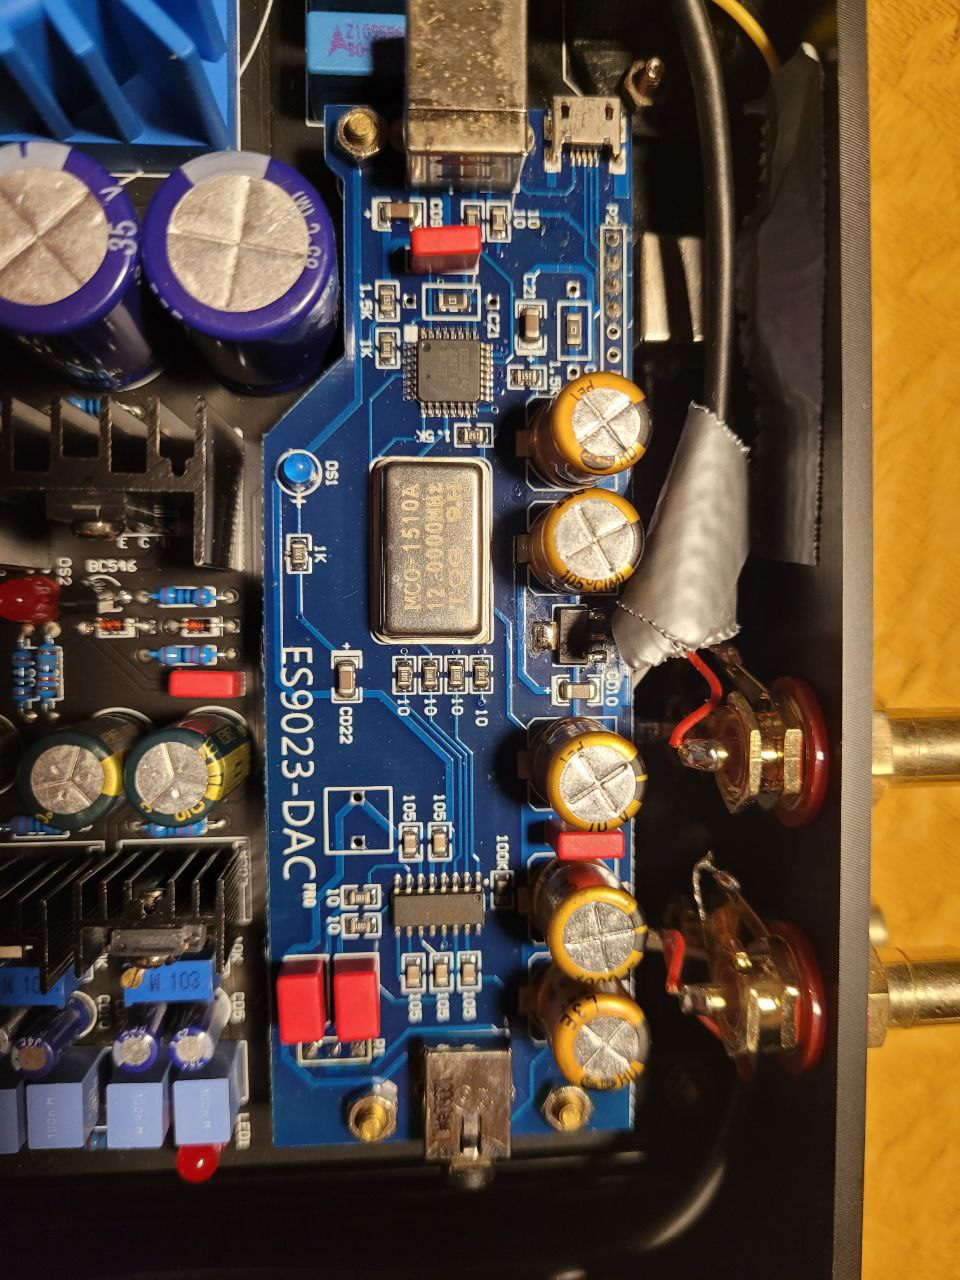
\includegraphics[width=0.7\textwidth, angle=90]{pictures/scheda-dac.png}
  \caption{Vista della scheda DAC ES9023 (modulo USB).}
  \label{fig:scheda-dac}
\end{figure}

L'hardware interno mostra:
\begin{itemize}
  \item un modulo blu con ricevitore USB--audio (classe \textbf{SA9023}),
        chip \textbf{ES9023} e oscillatore al quarzo da \SI{12}{MHz};
  \item un'alimentazione lineare con trasformatore toroidale YHDC PTC15,
        $2\times\SI{12}{V}/\SI{625}{mA}$;
  \item una scheda nera con amplificatore cuffie discreto su dissipatore;
  \item pannello posteriore con \emph{AUDIO IN}, \emph{AUDIO OUT} (RCA),
        USB-B e ingresso rete \SI{220}{V}.
\end{itemize}

\begin{figure}[H]
  \centering
  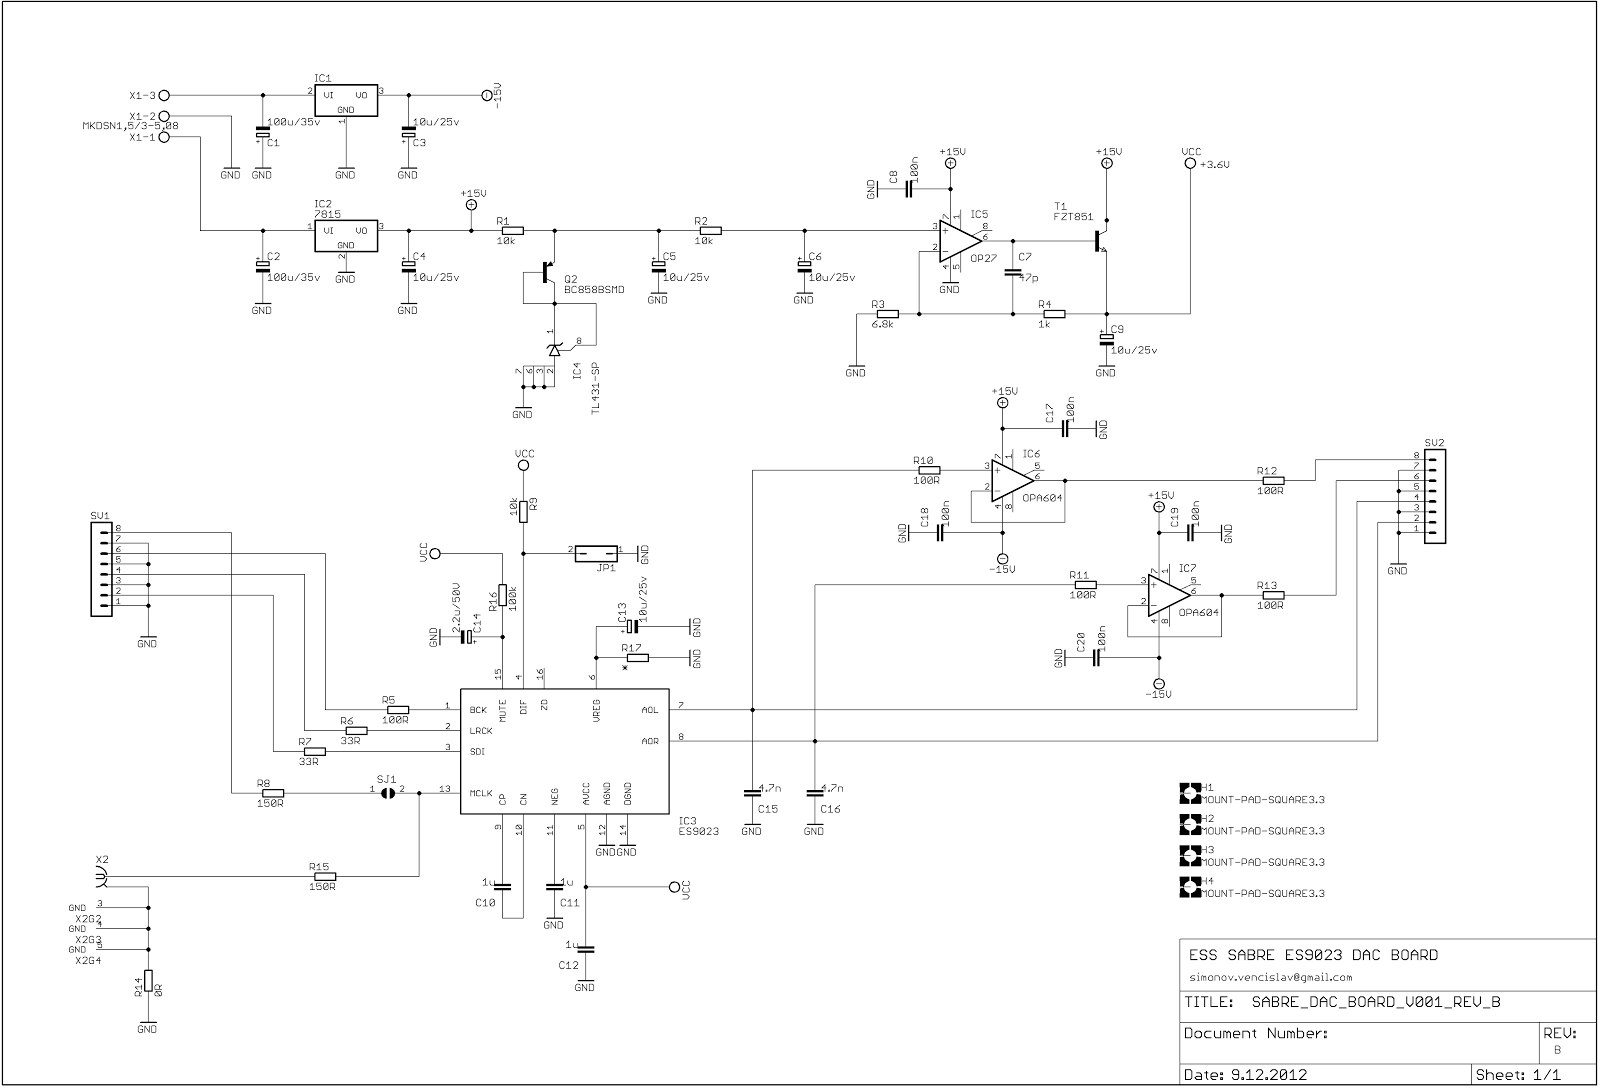
\includegraphics[width=0.7\textwidth]{pictures/ES9023_SCHEMATIC_DAC_AUDIO.png}
  \caption{Schematico di riferimento della sezione analogica ES9023
  (variante a ingresso I\textsuperscript{2}S di AudioWorkshop). Descrive
  bene la catena analogica del DAC ma \emph{non} è identico al front-end
  USB della scheda in esame.}
  \label{fig:circuito-dac}
\end{figure}

Lo schematico completo della variante I\textsuperscript{2}S è
disponibile online\footnote{\url{https://blog.audioworkshop.org/ess-es9023-sabre-dac-board/}};
specifiche e misure indipendenti dell'ES9023 sono reperibili su
AudioScienceReview\footnote{\url{https://www.audiosciencereview.com/forum/index.php?threads/dac-ess9023-decent-standard-measurements-very-poor-imd-does-that-make-sense.12639/}}.

Obiettivi del progetto:
\begin{enumerate}
  \item modellare i percorsi del segnale USB$\rightarrow$cuffie e
        USB$\rightarrow$RCA, inclusi gli stadi analogici;
  \item stimare guadagni, impedenze e rumore con i valori \emph{corretti}
        di guadagno ($\SI{18}{dB}$) e impedenza d'uscita ($\approx\SI{100}{\ohm}$);
  \item predisporre un modello SPICE parametrico per le simulazioni;
  \item analizzare il loop analogico IN$\rightarrow$OUT e proporre una
        modifica per pilotare lo stadio cuffie da una sorgente analogica (CD);
  \item determinare l'impedenza di cuffia ottimale e scegliere un modello.
\end{enumerate}

% =====================================================================
\section{Richiami teorici di segnali}\label{sec:teoria}
% =====================================================================
Questa sezione fornisce le basi formali usate nel resto del documento
(full scale, \si{dBFS}, clipping, dualità discreto/periodico, funzioni di
trasferimento LTI). È mantenuta sostanzialmente come nella stesura
originale; sono corretti un errore sulla corrispondenza fra frequenza
digitale e frequenza di Nyquist e qualche imprecisione di notazione fra
DFS e DFT.

\subsection{Definizione di full scale}
In relazione al segnale, il \emph{full-scale} è il punto di aggancio tra
il massimo numero digitale e la massima tensione analogica disponibile:
è il massimo livello analogico che il DAC può fornire quando il
\hyperref[sec:segnaleDigitale]{segnale digitale normalizzato} assume il
massimo valore ammesso. Quando $x[n]$ raggiunge tale valore, l'ES9023
fornisce la massima ampiezza analogica nominale. Non esistono livelli
superiori al full-scale: se il segnale digitale tentasse di superare il
limite $|x[n]|>1$ si avrebbe \emph{clipping} nel dominio digitale e
l'ampiezza dell'uscita analogica non potrebbe aumentare ulteriormente.

Quando si scrive che \SI{0}{dBFS} corrisponde a $|x[n]|=1$, si indica che
il campione digitale ha raggiunto il limite superiore della codifica,
oltre il quale si avrebbe \hyperref[sec:clipping]{clipping} digitale: non
è una tensione, non è una potenza, è un numero adimensionale, e l'intero
dominio digitale è contenuto in $[-1,1]$. Il passaggio al dominio
analogico avviene nel DAC, dove entra il concetto di full scale
analogico: se il datasheet riporta ``\SI{2}{V_{rms}} full scale'',
significa che una sinusoide digitale a \SI{0}{dBFS} produce in uscita una
sinusoide analogica con valore efficace pari a \SI{2}{V_{rms}}, sul carico
e nelle condizioni specificate dal costruttore.

\subsubsection{Segnale digitale normalizzato}\label{sec:segnaleDigitale}
Si definisce il segnale digitale normalizzato $x[n]$, con $|x[n]|\le1$,
dove $x[n]=\pm1$ corrisponde a \SI{0}{dBFS}. In digitale il full scale è
definito in termini di ampiezza massima assoluta, perché l'unità
\si{dBFS} misura il rapporto tra ampiezza attuale e ampiezza massima; per
questo sia $+1$ sia $-1$ rappresentano il picco massimo e corrispondono a
\SI{0}{dBFS}. Formalmente:
\begin{equation}
  \mathrm{dBFS}=20\log_{10}\!\left(\frac{|x[n]|}{x_{\max}}\right),
  \qquad x_{\max}=1,
\end{equation}
da cui $20\log_{10}(|\!\pm1|/1)=0\,\mathrm{dBFS}$. Definire $x[n]$ con
$|x[n]|\le1$ significa fissare un riferimento puramente numerico,
indipendente da qualunque tensione reale.

\subsubsection{Clipping}\label{sec:clipping}
Il clipping digitale è un troncamento immediato dei valori numerici,
mentre il clipping analogico è la saturazione fisica di un circuito. Il
primo è istantaneo: un campione viene tagliato al valore massimo o minimo
consentito, e genera armoniche molto alte (distorsione non lineare),
perché il troncamento introduce discontinuità nella forma d'onda; non
dipende da un carico elettrico. Il secondo dipende dall'elettronica: il
segnale è continuo e satura quando il circuito non può più produrre
tensioni maggiori (es.\ un amplificatore al limite di swing), con
transizione più morbida secondo le caratteristiche del circuito.

Il clipping digitale produce armoniche fino alla frequenza di Nyquist con
ampiezza significativa, causando aliasing se il segnale non è
oversampled. In analogico le armoniche decrescono rapidamente: la
distorsione è più contenuta nello spettro e non genera aliasing
intrinseco. La differenza chiave è la continuità della funzione di
trasferimento: il digitale introduce discontinuità istantanee (armoniche
forti e lunghe code spettrali); l'analogico una saturazione continua
(armoniche più morbide e decrescenti).

Considerando $x(t)$ continuo e la sua versione campionata $x[n]$ con
$|x[n]|\le1$, il clipping digitale si definisce come
\begin{equation}
  y[n]=
  \begin{cases}
    1, & x[n]>1\\
    x[n], & -1\le x[n]\le1\\
    -1, & x[n]<-1
  \end{cases}
\end{equation}
Il troncamento è immediato e produce discontinuità in $y[n]$; una
discontinuità netta nel tempo si traduce in contenuto spettrale molto
esteso in frequenza. Per $x[n]=\sin(\omega_0 n)$ normalizzato, il clipping
produce una funzione periodica non sinusoidale rappresentabile tramite
serie di Fourier discreta:
\begin{equation}
  y[n]=\sum_{k=0}^{N-1} Y[k]\,e^{j2\pi kn/N}.
\end{equation}
Un seno clippato simmetricamente attorno a zero è dispari
($y[-n]=-y[n]$), quindi la serie contiene solo armoniche dispari con
ampiezza decrescente come $1/k$, assimilabile a un'onda quadra
``morbida''\footnote{L'ampiezza delle armoniche decresce circa come $1/k$,
generando uno spettro simile a quello di un'onda quadra smussata; un
clipping più dolce decade più rapidamente del $1/k$ ideale.}:
\begin{equation}
  y[n]=\sum_{k=1,3,5,\dots}^{\infty} A_k\,\sin(k\omega_0 n).
\end{equation}

Il campionamento limita la frequenza massima rappresentabile a Nyquist,
\begin{equation}
  f_{\mathrm{N}}=\frac{f_s}{2}:
\end{equation}
nessuna informazione discreta può essere rappresentata sopra questa
frequenza senza aliasing; qualsiasi armonica reale che superi Nyquist
viene ripiegata in banda base. Anche senza oversampling\footnote{Con
l'oversampling si alza temporaneamente $f_s/2$: più armoniche restano
sopra la Nyquist originale ma sotto quella ``estesa'', quindi non
aliasano; applicando poi un low-pass e un downsample si eliminano le
armoniche alte prima che possano aliasare.}, le armoniche oltre Nyquist
generano aliasing. Non è l'oversampling a generare le armoniche, ma il
fatto che lo spettro del clipping vada oltre Nyquist; il decadimento
$1/k$ le riduce ma non le elimina.

In analogico non c'è limite di campionamento, quindi nessun aliasing. Un
circuito con saturazione sigmoide
\begin{equation}
  y(t)=f(x(t))=V_{\max}\tanh\!\left(\frac{x(t)}{V_{\max}}\right)
\end{equation}
ha derivata
\begin{equation}
  f'(x)=\frac{V_{\max}}{\cosh^2(x/V_{\max})}
\end{equation}
finita ovunque: niente discontinuità nel tempo, armoniche attenuate
(idealmente in modo esponenziale anziché $1/k$), suono più ``caldo''. Un
clipping analogico ``duro'' $y(t)=\mathrm{sgn}(x)\min(|x|,V_{\max})$ ha
derivata divergente agli estremi (cuspidi) e si avvicina al comportamento
del clipping digitale.

\paragraph{Serie di Fourier discreta e dualità.}\label{sec:fourier_duality}
La DFT si applica a un blocco finito di $N$ campioni, assunto discreto e
periodico; i coefficienti descrivono lo spettro discreto delle frequenze
di quel periodo. Intuizione di dualità:
\begin{itemize}
  \item \textbf{Discreto nel tempo $\rightarrow$ periodico in frequenza}:
        il campionamento equivale a moltiplicare per un treno di impulsi
        nel tempo, ossia a convolvere con impulsi periodici in frequenza,
        da cui spettro periodico.
  \item \textbf{Periodico nel tempo $\rightarrow$ discreto in frequenza}:
        la periodicità seleziona solo certe frequenze, da cui spettro
        discreto (righe).
\end{itemize}
Un segnale discreto e in generale non periodico ha DTFT
\begin{equation}
  X(e^{j\Omega})=\sum_{n=-\infty}^{\infty}x[n]\,e^{-j\Omega n},
\end{equation}
con $\Omega$ continua e spettro periodico di periodo $2\pi$. Prendendo un
blocco finito di $N$ campioni si valuta la DTFT in $N$ punti
equispaziati; assumendo per dualità il segnale periodico di periodo $N$,
si ottiene propriamente la \emph{serie di Fourier discreta} (DFS), che
coincide numericamente con la DFT:
\begin{equation}
  X[k]=\sum_{n=0}^{N-1}x[n]\,e^{-j2\pi kn/N},\qquad k=0,\dots,N-1,
  \label{eq:dft}
\end{equation}
con ricostruzione
\begin{equation}
  x[n]=\frac{1}{N}\sum_{k=0}^{N-1}X[k]\,e^{j2\pi kn/N},
  \qquad n\in\mathbb{Z}\ (\text{periodico modulo }N).
\end{equation}
La DFT tratta dunque il blocco finito come un periodo che si ripete: il
dominio della frequenza resta discreto e periodico, il che spiega perché
le armoniche del clipping digitale appaiano come righe discrete e
ripetute.

\paragraph{Serie di Fourier discreta, algebricamente.}
Sia $y[n]$ periodico di periodo $N$: $y[n+N]=y[n]$. Il vettore di un
periodo $y=[y[0],\dots,y[N-1]]^T$ vive in $\mathbb{C}^N$. Gli $N$ vettori
esponenziali complessi
\begin{equation}
  v_k=\big[\,e^{j2\pi k\cdot0/N},\,e^{j2\pi k\cdot1/N},\dots,
            e^{j2\pi k(N-1)/N}\,\big]^T,\quad k=0,\dots,N-1,
\end{equation}
sono linearmente indipendenti e formano una base ortogonale di
$\mathbb{C}^N$. Quindi ogni segnale periodico di lunghezza $N$ si scrive
come loro combinazione lineare
\begin{equation}
  y[n]=\sum_{k=0}^{N-1}Y[k]\,e^{j2\pi kn/N},
\end{equation}
dove $Y[k]$ sono i coefficienti della serie di Fourier discreta.

\subsubsection{Relazione tra \texorpdfstring{\si{dBFS}}{dBFS} e tensione RMS}
RMS (\emph{root mean square}) è una definizione energetica, non di picco.
Per un segnale periodico $v(t)$:
\begin{equation}
  V_{\mathrm{rms}}=\sqrt{\frac{1}{T}\int_0^T v^2(t)\,dt},
\end{equation}
e per una sinusoide pura $v(t)=V_p\sin(\omega t)$ vale
$V_{\mathrm{rms}}=V_p/\sqrt2$. Dire ``\SI{2}{V_{rms}} full scale'' implica
quindi un picco analogico $\approx2\sqrt2\,\si{V}$, salvo headroom
interni. L'RMS è la grandezza corretta perché legata direttamente alla
potenza su un carico resistivo, quindi all'SNR, alla dinamica e alla
distorsione misurabile.

\subsubsection{Funzioni di trasferimento ed esponenziali complessi}\label{sec:filter}
Il filtro digitale interno al DAC è un sistema LTI discreto: la risposta è
una convoluzione discreta, che per la proprietà LTI corrisponde a una
moltiplicazione in frequenza con $H(e^{j\Omega})$, anch'essa continua in
$\Omega$ e periodica di periodo $2\pi$. Operando su campioni
$x[n]=x_c(nT_s)$, la frequenza naturale è quella digitale normalizzata
$\Omega$, legata alla frequenza continua da
\begin{equation}
  \Omega=\omega T_s=2\pi f T_s .
\end{equation}

\paragraph{Correzione rispetto alla stesura originale.} Un ciclo completo
in frequenza digitale, $\Omega=2\pi$, corrisponde a $f=1/T_s=f_s$, cioè la
\emph{frequenza di campionamento}; la frequenza di \textbf{Nyquist}
$f_{\mathrm{N}}=f_s/2$ corrisponde invece a $\Omega=\pi$. (Nella versione
precedente $\Omega=2\pi$ era erroneamente associata a $f_s/2$.)

Confrontando con la \eqref{eq:dft}, il $k$-esimo punto della DFT cade a
\begin{equation}
  \Omega_k=\frac{2\pi k}{N}\ \text{(rad/campione)},\qquad
  f_k=\frac{k}{NT_s}\ \xrightarrow{T_s=1}\ \frac{k}{N}.
\end{equation}

Per un sistema LTI discreto, gli esponenziali complessi $e^{j\Omega n}$
sono autofunzioni. Se $x[n]=e^{j\Omega n}$ entra in un sistema con
risposta all'impulso $h[n]$:
\begin{equation}
  y[n]=\sum_{k=-\infty}^{\infty}h[k]\,e^{j\Omega(n-k)}
      =e^{j\Omega n}\sum_{k=-\infty}^{\infty}h[k]\,e^{-j\Omega k}
      =H(e^{j\Omega})\,e^{j\Omega n}.
\end{equation}
L'uscita è l'ingresso scalato da $H(e^{j\Omega})$: per definizione la
risposta in frequenza del filtro digitale. La notazione
$H_D(e^{j\Omega})$ corrisponde a valutare la trasformata Z
\begin{equation}
  H(z)=\sum_{n=-\infty}^{\infty}h[n]\,z^{-n},\qquad z\in\mathbb{C},
\end{equation}
sulla circonferenza unitaria $z=e^{j\Omega}$:
$H_D(e^{j\Omega})=H(z)\big|_{z=e^{j\Omega}}$. La DTFT è dunque un caso
particolare della trasformata Z, e la valutazione su $|z|=1$ è proprio ciò
che dà la risposta in frequenza, coerentemente con il ruolo di
autofunzione degli esponenziali complessi.

Il filtro analogico post-DAC è invece LTI continuo, con autofunzioni
$e^{j\omega t}$: se $v(t)=e^{j\omega t}$ allora
$y(t)=H_A(j\omega)\,e^{j\omega t}$, dove $H_A(j\omega)$ è la trasformata di
Laplace valutata su $s=j\omega$. Digitale e analogico vivono quindi in
spazi di frequenza distinti ma collegati: $H_D(e^{j\Omega})$ modella
interpolazione, imaging e roll-off prima della conversione D/A;
$H_A(j\omega)$ il filtraggio anti-imaging reale, i limiti di banda, fase e
distorsione dopo. Scriverli come prodotto è corretto perché entrambi LTI,
quindi concatenabili per moltiplicazione delle risposte in frequenza, una
volta fissato il mapping $\Omega\leftrightarrow\omega$.

% =====================================================================
\section{Architettura del sistema (rivista)}
% =====================================================================

\subsection{Blocchi funzionali reali}
Il dispositivo è composto da tre sottosistemi fisicamente distinti:
\begin{itemize}
  \item \textbf{Modulo USB--DAC} (scheda blu ``ES9023-DAC''): ricevitore
        USB--audio SA9023 + quarzo \SI{12}{MHz} + ES9023 + filtro RC
        d'uscita. Fornisce due canali \emph{line-level} a $\approx\SI{2}{V_{rms}}$.
  \item \textbf{Stadio amplificatore cuffie discreto} (scheda nera):
        transistor su dissipatore, trimmer di bias, alimentazione duale.
        Topologia A1-like: voltage-oriented, alta impedenza d'uscita.
  \item \textbf{Alimentazione lineare}: toroide YHDC PTC15
        ($2\times\SI{115}{V}$ primari in serie per rete \SI{230}{V};
        $2\times\SI{12}{V}/\SI{625}{mA}$ secondari), raddrizzamento +
        regolatori lineari (es.\ 7812/7912) per i rail dello stadio
        cuffie; LDO dedicato a bordo della scheda blu per il DAC.
\end{itemize}

\subsection{Percorsi del segnale}
Con $x[n]$ segnale digitale normalizzato ($|x[n]|\le1$, $0\,\mathrm{dBFS}\equiv|x[n]|=1$)
e $V_{\mathrm{FS}}\approx\SI{2}{V_{rms}}$ il full-scale del DAC:
\begin{align}
  V_{\text{LINE}}(j\omega) &=
     V_{\mathrm{FS}}\,X(e^{j\Omega})\,H_{B}(e^{j\Omega})\,H_{D}(e^{j\Omega})\,H_{A}(j\omega), \\[2pt]
  V_{\text{HP}}(j\omega) &=
     V_{\text{LINE}}(j\omega)\,H_{\text{vol}}\,H_{HP}(j\omega)\,
     \underbrace{\frac{R_L}{R_L+Z_{\text{out}}}}_{\text{partitore d'uscita}} ,
\end{align}
dove rispetto alla versione precedente compaiono esplicitamente:
$H_B$ (ricevitore USB SA9023, jitter/clock domain), $H_{\text{vol}}$
(potenziometro ALPS) e soprattutto il \textbf{partitore d'uscita}
$R_L/(R_L+Z_{\text{out}})$, che con $Z_{\text{out}}\approx\SI{100}{\ohm}$
\emph{non} è trascurabile. La giustificazione strutturale (gli
esponenziali complessi come autofunzioni dei sistemi LTI discreti e
continui, da cui la concatenabilità per moltiplicazione delle risposte
in frequenza) resta quella già sviluppata nei richiami teorici.

Il loop analogico \emph{AUDIO IN}$\rightarrow$\emph{AUDIO OUT} si modella
come passthrough passivo:
\begin{equation}
  V_{\text{OUT,loop}}(j\omega)\approx V_{\text{IN,loop}}(j\omega)\,H_{\text{loop}}(j\omega),
  \qquad H_{\text{loop}}\approx 1 .
\end{equation}

\begin{figure}[H]
  \centering
  \begin{circuitikz}[american voltages]
    \draw (0,0)  node[draw,minimum width=2.1cm,minimum height=1cm] (usb)  {USB-B};
    \draw (2.9,0)node[draw,minimum width=2.1cm,minimum height=1cm] (sa)   {SA9023};
    \draw (5.8,0)node[draw,minimum width=2.1cm,minimum height=1cm] (dac)  {ES9023};
    \draw (8.7,0)node[draw,minimum width=2.1cm,minimum height=1cm] (amp)  {Amp cuffie};
    \draw (11.4,0)node[draw,minimum width=1.7cm,minimum height=0.9cm] (hp){Cuffie};
    \draw (5.8,-2.2)node[draw,minimum width=2.1cm,minimum height=1cm] (in){RCA IN};
    \draw (8.7,-2.2)node[draw,minimum width=2.1cm,minimum height=1cm] (out){RCA OUT};
    \draw[->] (usb)--(sa) node[midway,above]{USB};
    \draw[->] (sa)--(dac) node[midway,above]{I\textsuperscript{2}S};
    \draw[->] (dac)--(amp) node[midway,above]{$\SI{2}{V_{rms}}$};
    \draw[->] (amp)--(hp);
    \draw[->] (in)--(out) node[midway,above]{loop passivo};
    \draw[densely dashed,->] (dac.south) |- (out.west) node[pos=0.75,above]{? (da verificare)};
  \end{circuitikz}
  \caption{Architettura rivista. Linea tratteggiata: collegamento
  DAC$\rightarrow$RCA~OUT \emph{ipotetico}, da confermare con la misura di
  Sez.~\ref{sec:misure}.}
  \label{fig:arch}
\end{figure}

% =====================================================================
\section{Punto (a): instradamento di RCA IN, RCA OUT e cuffie}\label{sec:routing}
% =====================================================================

\subsection{Domanda e ipotesi}
La domanda è duplice: (i) lo \emph{stesso} segnale può raggiungere
contemporaneamente le cuffie e una coppia di casse attive sull'RCA~OUT?
(ii) oppure l'RCA~OUT è soltanto un \emph{passthrough} dell'RCA~IN
analogico?

Nella topologia A1 di riferimento l'uscita RCA è esplicitamente un
\emph{loop passivo} dell'ingresso (``RCA in directly to the RCA out''),
attivo anche a dispositivo spento, pensato per inviare la sorgente a un
amplificatore stereo o a casse attive. Se il telaio conserva questa
topologia, allora:
\begin{itemize}
  \item \textbf{RCA~OUT $=$ copia passiva di RCA~IN} (analogico), \emph{indipendente} dal DAC;
  \item il \textbf{DAC alimenta solo lo stadio cuffie} (cablaggio interno
        al nodo d'ingresso dell'amp), non l'RCA~OUT.
\end{itemize}
Questa è la conclusione \emph{opposta} a quella della bozza iniziale, che
assumeva l'RCA~OUT pilotato dal nodo analogico del DAC. Esiste però la
variante di modifica in cui l'integratore ha cablato l'uscita del DAC
\emph{anche} all'RCA~OUT: in tal caso il DAC pilota sia cuffie sia casse.
Entrambe sono topologie reali su apparecchi di questo tipo; solo la
misura decide.

\subsection{Conseguenze elettriche}
Se l'RCA~OUT è il \SI{2}{V_{rms}} del DAC (uscita ES9023 con
$R_{\text{out,int}}\approx\SI{200}{\ohm}$ + serie \SI{22}{\ohm}), su un
ingresso linea da \SI{10}{k\ohm} l'attenuazione è
\begin{equation}
  A_{\text{line}}\approx\frac{10\,000}{10\,000+222}\approx0.978\;(\approx\SI{-0.19}{dB}),
\end{equation}
trascurabile: il DAC pilota bene casse attive o un finale. Se invece è il
loop passivo dell'RCA~IN, l'RCA~OUT riproduce semplicemente la sorgente
collegata in ingresso, a guadagno unitario.

\subsection{Verifica sperimentale}\label{sec:misure}
\textbf{Test di instradamento RCA~OUT} (multimetro in AC volt o
oscilloscopio):
\begin{enumerate}
  \item Riproduci dal PC un tono sinusoidale a \SI{1}{kHz},
        $\approx\SI{-6}{dBFS}$, tramite USB. Misura la tensione AC tra
        centrale e massa dell'RCA~OUT.
        \begin{itemize}
          \item Segnale presente e proporzionale al volume di sistema
                $\Rightarrow$ \emph{il DAC è cablato all'RCA~OUT}.
          \item RCA~OUT silenzioso $\Rightarrow$ non è alimentato dal DAC.
        \end{itemize}
  \item Inietta un segnale noto sull'RCA~IN e rimisura l'RCA~OUT: se
        ricompare a guadagno $\approx1$, l'RCA~OUT è il \emph{loop} di RCA~IN.
  \item \textbf{Firma A1}: spegni l'unità lasciando la sorgente
        sull'RCA~IN. Se l'RCA~OUT continua a passare il segnale a unità
        spenta, è confermato il loop passivo (l'A1 lo fa per progetto).
\end{enumerate}

% =====================================================================
\section{Punto (b): natura della customizzazione}\label{sec:custom}
% =====================================================================

\subsection{Punto di partenza (A1 o clone A1-like)}
L'amplificatore di base è un \emph{headphone amp} analogico discreto,
class-A/AB, voltage-oriented, con potenziometro ALPS, alimentazione
lineare toroidale e finale su dissipatore. Non integra DAC né DSP:
riceve un segnale \emph{line-level} e lo amplifica. Caratteristiche A1
documentate: risposta \SIrange{1}{100}{kHz}, range cuffie
\SIrange{30}{600}{\ohm}, $Z_{\text{out}}\approx\SI{100}{\ohm}$, guadagno
max \SI{18}{dB}, due ingressi RCA con selettore a relè, una uscita RCA in
loop, un jack cuffie.

\subsection{Modifica effettuata}
La customizzazione consiste nel \textbf{sostituire la sorgente analogica
con un modulo USB-DAC interno}:
\begin{enumerate}
  \item è stato aggiunto un connettore \textbf{USB-B} sul pannello
        posteriore, cablato (spesso via micro-USB interno) alla scheda blu;
  \item la scheda \textbf{SA9023+ES9023} enumera sotto Windows come
        scheda audio USB (UAC, tipicamente fino a \SI{24}{bit}/\SI{96}{kHz}
        col SA9023) e fornisce \SI{2}{V_{rms}} line-level;
  \item questo line-level è \textbf{cablato internamente al nodo
        d'ingresso dello stadio cuffie}, in sostituzione (o in parallelo)
        di uno degli ingressi RCA originali;
  \item il loop \textbf{RCA~IN$\rightarrow$RCA~OUT} è verosimilmente
        rimasto invariato (vedi punto (a)).
\end{enumerate}
La riduzione da due ingressi RCA (A1) a un solo \emph{AUDIO IN} sul
pannello, più i \emph{due} jack cuffie osservati, indicano un lavoro di
integrazione di piccola scala (laboratorio/OEM asiatico), non una
revisione ufficiale Beyerdynamic: l'A1 di fabbrica non è mai stato
venduto con DAC USB e ha un solo jack cuffie. L'attribuzione ``A1'' va
quindi intesa come \emph{topologia di riferimento}, non come certificato
d'origine.

% =====================================================================
\section{Stadio DAC ES9023 (scheda USB)}
% =====================================================================

\subsection{Specifiche rilevanti}
\begin{table}[H]
  \centering
  \begin{tabular}{ll}
    \toprule
    Parametro & Valore (datasheet/board) \\
    \midrule
    Architettura      & SABRE HyperStream, charge pump interno \\
    Risoluzione        & \SI{24}{bit}, fino a \SI{192}{kHz} (DAC) \\
    Uscita full-scale  & $\approx\SI{2}{V_{rms}}$ (regolabile in basso con R esterna) \\
    Dynamic range/SNR  & fino a \SI{112}{dB} \\
    THD+N tipico       & $\sim\SI{0.002}{\%}$ \\
    Uscita             & riferita a massa, \emph{senza} cap di blocco DC \\
    Front-end USB      & SA9023-class, UAC fino a \SI{24}{bit}/\SI{96}{kHz} \\
    \bottomrule
  \end{tabular}
  \caption{Sintesi delle specifiche ES9023 + ricevitore USB.}
\end{table}

\subsection{Filtro RC post-DAC}
Filtro del primo ordine con $R_s=\SI{22}{\ohm}$, $C_f=\SI{4.7}{nF}$:
\begin{equation}
  H_A(s)=\frac{1}{1+sR_sC_f},\qquad
  f_c=\frac{1}{2\pi R_sC_f}\approx\SI{1.54}{MHz}.
\end{equation}
Ben oltre la banda audio: serve solo a sopprimere i residui di
modulazione del DAC. Nessun effetto udibile.

\subsection{Alimentazione del DAC}
Sulla \emph{tua} scheda USB la \SI{3.6}{V} (o \SI{3.3}{V}) per l'ES9023 è
generata da un LDO a basso rumore a bordo, non dalla rete TL431+OPA604
dello schematico AudioWorkshop. Il principio (riferimento stabile +
filtro passa-basso a frazioni di hertz) è analogo; l'ordine di grandezza
del rumore in banda audio resta sub-\si{\micro V_{rms}}, ampiamente sotto
il floor del DAC. L'analisi che segue si riferisce alla
\emph{variante I\textsuperscript{2}S/AudioWorkshop} con regolatore TL431
(Fig.~\ref{fig:circuito-dac}); è riportata per completezza e fornisce un
limite superiore al rumore d'alimentazione, dato che l'LDO integrato
della scheda USB tipicamente fa meglio.

\subsubsection{Regolatore low-noise basato su TL431}
Il TL431 genera un riferimento $V_{\text{ref}}\approx\SI{2.5}{V}$,
successivamente partito/amplificato. In DC:
\begin{equation}
  V_{\text{out}}=V_{\text{ref}}\left(1+\frac{R_3}{R_4}\right),
  \qquad \frac{R_3}{R_4}\approx0.44 \Rightarrow V_{\text{out}}\approx\SI{3.6}{V}.
\end{equation}

\subsubsection{Filtro \texorpdfstring{$R_2$--$C_6$}{R2-C6} sul riferimento}
Un passa-basso del primo ordine filtra il rumore del riferimento:
\begin{equation}
  H_{\text{ref}}(s)=\frac{1}{1+sR_2C_6},\qquad
  f_{c,\text{ref}}=\frac{1}{2\pi R_2C_6}.
\end{equation}
Con $R_2=\SI{1}{k\ohm}$ e $C_6=\SI{100}{\micro\farad}$:
$f_{c,\text{ref}}\approx\SI{1.6}{Hz}$, quindi il rumore del TL431 è
fortemente attenuato già sopra pochi hertz (a \SI{20}{Hz} la reiezione è
$\sim\SI{20}{dB}$).

\subsubsection{Rumore del regolatore}
Trascurando il TL431 dopo il filtro e considerando il rumore dell'op-amp
$e_{n,\text{op}}\approx\SI{4}{nV/\sqrt{Hz}}$, la densità riferita
all'uscita è
\begin{equation}
  e_{n,\text{out}}\approx\left(1+\frac{R_3}{R_4}\right)e_{n,\text{op}}
  \approx1.44\times\SI{4}{nV/\sqrt{Hz}}\approx\SI{5.7}{nV/\sqrt{Hz}}.
\end{equation}
Integrando su $B\approx\SI{20}{kHz}$:
\begin{equation}
  e_{\text{out,rms}}\approx e_{n,\text{out}}\sqrt{B}\approx\SI{0.8}{\micro V_{rms}}.
\end{equation}
Rapporto rispetto al full-scale del DAC ($\SI{2}{V_{rms}}$):
\begin{equation}
  \text{SNR}_{\text{PSU}}=20\log_{10}\!\left(\frac{2}{0.8\cdot10^{-6}}\right)
  \approx\SI{128}{dB}.
\end{equation}
Il contributo dell'alimentazione è dunque ampiamente sotto il limite
imposto dal DAC stesso ($\sim\SI{112}{dB}$): non è il collo di bottiglia.

% =====================================================================
\section{Filtro di accoppiamento in AC}\label{sec:accoppiamento}
% =====================================================================
L'uscita dell'ES9023 è riferita a massa e \emph{non} richiede
condensatori di blocco DC (grazie al charge pump interno). Eventuali
condensatori di accoppiamento compaiono quindi non all'uscita del DAC, ma
nei punti di interfaccia interni: l'accoppiamento del line-level verso il
nodo d'ingresso dello stadio cuffie e l'eventuale ingresso analogico CD.
Ciascuno realizza un passa-alto del primo ordine.

\subsection{Passa-alto \texorpdfstring{$C_c$--$R_{\text{load}}$}{Cc-Rload}}
\begin{equation}
  H_{\text{HP}}(s)=\frac{sR_{\text{load}}C_c}{1+sR_{\text{load}}C_c},
  \qquad f_{\text{HP}}=\frac{1}{2\pi R_{\text{load}}C_c}.
\end{equation}
Verso un ingresso linea con $R_{\text{load}}=\SI{22}{k\ohm}$ e
$C_c=\SI{4.7}{\micro\farad}$:
\begin{equation}
  f_{\text{HP}}\approx\frac{1}{2\pi\cdot22\,000\cdot4.7\cdot10^{-6}}\approx\SI{1.5}{Hz},
\end{equation}
quindi la banda \SIrange{20}{20000}{Hz} è coperta con perdita a
\SI{20}{Hz} inferiore a \SI{0.1}{dB}.

\subsection{Accoppiamento verso lo stadio cuffie}
Se l'ingresso del pre cuffie ha $R_{\text{in,HP}}\approx\SI{47}{k\ohm}$ con
lo stesso $C_c=\SI{4.7}{\micro\farad}$:
\begin{equation}
  f_{\text{HP,HP}}=\frac{1}{2\pi R_{\text{in,HP}}C_c}\approx\SI{0.7}{Hz},
\end{equation}
del tutto trascurabile rispetto alla banda audio. Anche il percorso
CD$\rightarrow$cuffie ha quindi risposta in bassa frequenza piena e
lineare.

% =====================================================================
\section{Stadio cuffie discreto (modello rivisto)}
% =====================================================================

\subsection{Guadagno e swing}
Adottando il dato A1 di guadagno massimo \SI{18}{dB} ($\approx 7.9\times$)
anziché i \SI{12}{dB} assunti in precedenza:
\begin{equation}
  G_{HP,\max}\approx 10^{18/20}\approx 7.9,\qquad
  V_{\text{HP,teor}}=G_{HP,\max}\,V_{\mathrm{FS}}\approx 7.9\times\SI{2}{V_{rms}}\approx\SI{16}{V_{rms}}.
\end{equation}
Questo valore è puramente nominale: lo swing reale è limitato dai rail.
Con rail $\pm\SIrange{12}{15}{V}$ il massimo prima del clipping è
\begin{equation}
  V_{\text{HP,max}}\approx\frac{V_{\text{rail}}-V_{\text{sat}}}{\sqrt 2}
  \approx\frac{14}{\sqrt 2}\approx\SI{9.9}{V_{rms}}\;(\text{rail }\pm\SI{15}{V}).
\end{equation}
Il guadagno alto significa solo che si raggiunge il fondo scala con la
manopola ben sotto il massimo; il livello d'ascolto si imposta col
potenziometro. Il valore di lavoro $\approx\SIrange{5}{8}{V_{rms}}$ usato
nei conti di potenza resta valido.

\subsection{Impedenza d'uscita: la correzione decisiva}\label{sec:zout}
La versione precedente assumeva un emitter-follower con
$Z_{\text{out}}\approx\SI{1}{\ohm}$. Nella topologia A1 la realtà è
$Z_{\text{out}}\approx\SI{100}{\ohm}$ (resistenza serie d'uscita
deliberata). Conseguenze su una cuffia di impedenza $R_L$:
\begin{equation}
  V_{R_L}=V_{\text{amp}}\,\frac{R_L}{R_L+Z_{\text{out}}},\qquad
  DF=\frac{R_L}{Z_{\text{out}}} .
\end{equation}

\begin{table}[H]
  \centering
  \begin{tabular}{rccc}
    \toprule
    $R_L$ (\si{\ohm}) & Partitore $R_L/(R_L+100)$ & Perdita (\si{dB}) & $DF=R_L/100$ \\
    \midrule
    32  & 0.24 & $-12.3$ & 0.32 \\
    80  & 0.44 & $-7.1$  & 0.80 \\
    250 & 0.71 & $-2.9$  & 2.50 \\
    300 & 0.75 & $-2.5$  & 3.00 \\
    600 & 0.86 & $-1.3$  & 6.00 \\
    \bottomrule
  \end{tabular}
  \caption{Effetto di $Z_{\text{out}}=\SI{100}{\ohm}$. Le basse impedenze
  perdono molto livello e hanno fattore di smorzamento $<1$.}
  \label{tab:zout}
\end{table}

Il problema non è solo la perdita di livello: poiché l'impedenza di una
cuffia dinamica \emph{varia con la frequenza} (picco di risonanza in
gamma bassa), un'alta $Z_{\text{out}}$ trasforma quella variazione in una
\textbf{colorazione tonale} (tipicamente un rialzo dei bassi al picco di
risonanza). Questo spiega il carattere ``punchy'' e la raccomandazione di
usare cuffie ad \emph{alta} impedenza e con curva d'impedenza
relativamente piatta.

\subsection{Potenza utile (con partitore)}
La potenza dissipata nella cuffia è $P_L=V_{R_L}^2/R_L$ con
$V_{R_L}=V_{\text{amp}}\,R_L/(R_L+Z_{\text{out}})$. Per
$V_{\text{amp}}=\SI{5}{V_{rms}}$ a monte del partitore:

\begin{table}[H]
  \centering
  \begin{tabular}{rccc}
    \toprule
    $R_L$ (\si{\ohm}) & $V_{R_L}$ (\si{V_{rms}}) & $P_L$ con $Z_{\text{out}}=\SI{100}{\ohm}$ & $P_L$ con $Z_{\text{out}}=\SI{1}{\ohm}$ \\
    \midrule
    32  & 1.21 & \SI{46}{mW}  & \SI{780}{mW} \\
    80  & 2.22 & \SI{62}{mW}  & \SI{309}{mW} \\
    300 & 3.75 & \SI{47}{mW}  & \SI{83}{mW}  \\
    600 & 4.29 & \SI{31}{mW}  & \SI{42}{mW}  \\
    \bottomrule
  \end{tabular}
  \caption{Potenza utile in funzione di $Z_{\text{out}}$. Il caso
  \SI{100}{\ohm} (A1-like) penalizza pesantemente le basse impedenze; per
  alta impedenza la differenza è contenuta.}
\end{table}

Anche con \SI{31}{mW} su \SI{600}{\ohm} il livello è abbondante: su una
cuffia da $\sim\SI{96}{dB/mW}$ si superano \SI{110}{dB} SPL. Per le alte
impedenze, dunque, l'apparecchio resta pienamente adeguato \emph{a
prescindere} dal valore esatto di $Z_{\text{out}}$.

% =====================================================================
\section{Carichi cuffia e cuffie in parallelo (corretto)}\label{sec:carichi}
% =====================================================================
Il carico visto dall'amplificatore dipende dal numero di cuffie collegate
(i due jack frontali) e dalla loro impedenza. Tutti i conti che seguono
includono ora il partitore d'uscita $R_L/(R_L+Z_{\text{out}})$ con
$Z_{\text{out}}\approx\SI{100}{\ohm}$ (correzione rispetto alla versione
che assumeva $Z_{\text{out}}\approx\SI{1}{\ohm}$).

\subsection{Cuffia singola}
Detta $V_{\text{amp}}$ la tensione a monte del partitore, la tensione
effettiva e la potenza al carico sono
\begin{equation}
  V_{R_L}=V_{\text{amp}}\frac{R_L}{R_L+Z_{\text{out}}},\qquad
  P_L=\frac{V_{R_L}^2}{R_L}.
\end{equation}
I valori numerici (per $V_{\text{amp}}=\SI{5}{V_{rms}}$) sono in
Tab.~\ref{tab:zout} e nella tabella di potenza della
Sez.~\ref{sec:zout}: si noti che, a differenza del caso ideale
$Z_{\text{out}}\approx\SI{1}{\ohm}$, le basse impedenze non beneficiano
più della maggior potenza, perché il partitore le penalizza.

\subsection{Due cuffie in parallelo}
Con due cuffie identiche $R_{L1}=R_{L2}=R_L$ l'impedenza vista è
\begin{equation}
  R_{\text{eq}}=\frac{R_{L1}R_{L2}}{R_{L1}+R_{L2}}=\frac{R_L}{2}.
\end{equation}
Per due cuffie da \SI{32}{\ohm}: $R_{\text{eq}}=\SI{16}{\ohm}$. Con
$Z_{\text{out}}=\SI{100}{\ohm}$ il partitore diventa $16/116\approx0.14$:
oltre \SI{-17}{dB} di perdita di livello, oltre alla colorazione. \`E la
conferma quantitativa che \textbf{collegare due cuffie a bassa impedenza è
sconsigliato} su questo amplificatore. Con due cuffie da \SI{300}{\ohm}
($R_{\text{eq}}=\SI{150}{\ohm}$) il partitore $150/250=0.6$ resta
gestibile.

La corrente richiesta raddoppia rispetto alla singola cuffia,
$I_{\text{out}}=V/R_{\text{eq}}=2V/R_L$, ricordando che il toroide da
$\approx\SI{15}{VA}$ limita la corrente: ulteriore ragione per preferire
l'alta impedenza, specie con due uscite in uso.

\subsection{Fattore di smorzamento (corretto)}
Con $Z_{\text{out}}\approx\SI{100}{\ohm}$:
\begin{equation}
  DF=\frac{R_L}{Z_{\text{out}}}=
  \begin{cases}
    32/100=0.32 & (R_L=\SI{32}{\ohm})\\[2pt]
    300/100=3.0 & (R_L=\SI{300}{\ohm})\\[2pt]
    600/100=6.0 & (R_L=\SI{600}{\ohm}).
  \end{cases}
\end{equation}
Questi valori sostituiscono il $DF\approx32$ della stesura precedente
(che presupponeva $Z_{\text{out}}\approx\SI{1}{\ohm}$). Un $DF<1$ sulle
basse impedenze, oltre a indicare scarso controllo, implica forte
dipendenza della risposta dalla curva d'impedenza della cuffia. \`E,
ancora una volta, l'argomento dirimente a favore delle cuffie ad alta
impedenza, e dipende dalla misura di $Z_{\text{out}}$
(Sez.~\ref{sec:zout-mis}): se l'apparecchio fosse un clone con
$Z_{\text{out}}\approx\SI{1}{\ohm}$, i $DF$ tornerebbero elevati e il
quadro cambierebbe.

% =====================================================================
\section{Rumore complessivo (aggiornato)}
% =====================================================================
Rumore del DAC riferito all'uscita linea (DR $\approx\SI{112}{dB}$,
$V_{\mathrm{FS}}=\SI{2}{V_{rms}}$):
\begin{equation}
  V_{n,\text{DAC}}=V_{\mathrm{FS}}\,10^{-112/20}\approx\SI{5}{\micro V_{rms}}.
\end{equation}
Portato all'uscita amp con guadagno effettivo $G$ (a volume tale da avere
$\approx\SI{5}{V_{rms}}$, quindi $G\approx2.5$) e poi al carico tramite il
partitore di Tab.~\ref{tab:zout}:
\begin{equation}
  V_{n,\text{out}}\approx G\,V_{n,\text{DAC}}\,\frac{R_L}{R_L+Z_{\text{out}}}.
\end{equation}
Il rumore proprio dell'amp ($e_n\sqrt{B}$ con
$e_n\approx\SI{5}{nV/\sqrt{Hz}}$, $B=\SI{20}{kHz}$) somma in quadratura.
Il risultato resta nell'ordine della decina di \si{\micro V_{rms}} al
carico: con un floor così basso, su cuffie ad alta impedenza il fruscio è
inudibile e il dynamic range pratico è limitato dal DAC ($\sim\SI{112}{dB}$),
non dall'amplificatore.

% =====================================================================
\section{Alimentazione lineare}
% =====================================================================
Toroide YHDC PTC15: $2\times\SI{12}{V}/\SI{625}{mA}$, ovvero
$\approx\SI{7.5}{VA}$ per avvolgimento, $\approx\SI{15}{VA}$ totali. Con i
due secondari per le due polarità:
\begin{equation}
  V_{\text{DC,picco}}\approx\sqrt2\cdot\SI{12}{V}-2V_{\!D}\approx\SI{15.5}{V},
\end{equation}
da cui rail regolati $\pm\SI{12}{V}$ (7812/7912) oppure uso quasi-non
regolato a $\approx\pm\SI{15}{V}$. La corrente media disponibile
($\sim\SI{600}{mA}$ di picco per ramo) è coerente con un amp
\emph{voltage-oriented} per alta impedenza: abbondante in tensione,
limitato in corrente. È un'ulteriore conferma che il punto debole sono le
\emph{basse} impedenze ad alto volume, non le alte.

% =====================================================================
\section{Ingresso analogico RCA e modifica CD\texorpdfstring{$\rightarrow$}{->}cuffie}\label{sec:ingresso}
% =====================================================================
Lo stadio \emph{AUDIO IN}$\rightarrow$\emph{AUDIO OUT} si comporta, nella
topologia A1, come loop passivo: l'attenuazione su un ingresso tipico da
\SI{10}{k\ohm} è $\approx\SI{0.2}{dB}$, e il segnale resta presente
all'uscita RCA anche a unità spenta (vedi punto (a),
Sez.~\ref{sec:routing}). In configurazione di fabbrica questo loop
\emph{non} è collegato allo stadio cuffie.

\subsection{Modifica proposta: selettore DAC/CD verso le cuffie}
Per ascoltare in cuffia anche una sorgente analogica (es.\ un lettore CD
sull'\emph{AUDIO IN}), si può aggiungere un selettore che instrada al
nodo d'ingresso del pre cuffie o il line-level del DAC o il segnale CD:
\begin{equation}
  v_{\text{hp\_in}}=(1-\text{SEL})\,v_{\text{line}}+\text{SEL}\,v_{\text{cd\_line}},
  \qquad \text{SEL}\in\{0,1\}.
\end{equation}
Con \texttt{SEL=0} si ascolta il DAC USB, con \texttt{SEL=1} il CD.
Implementazione consigliata: relè di segnale o deviatore di buona qualità
sul nodo d'ingresso (impedenza $\sim\SI{47}{k\ohm}$), mantenendo il
condensatore di accoppiamento da \SI{4.7}{\micro\farad} già dimensionato
in Sez.~\ref{sec:accoppiamento} ($f_{\text{HP}}\approx\SI{0.7}{Hz}$, banda
piena). Il loop RCA~IN$\rightarrow$RCA~OUT può restare invariato.

\subsection{Avvertenza di livello}
Sorgente CD e DAC sono entrambi $\approx\SI{2}{V_{rms}}$ full-scale: con
il guadagno \SI{18}{dB} dello stadio cuffie, il potenziometro ALPS va
tenuto ben sotto il massimo per evitare il clipping ai rail
(Sez.~\ref{sec:zout}). Non sono necessari adattamenti di livello fra le
due sorgenti.

% =====================================================================
\section{Punto (c): impedenza pilotabile e scelta della cuffia}\label{sec:cuffie}
% =====================================================================

\subsection{Qual è la ``massima impedenza pilotabile''?}
La domanda va capovolta. Per un amplificatore l'alta impedenza è
\emph{facile}: richiede tensione, non corrente. Con rail $\pm\SIrange{12}{15}{V}$
e guadagno \SI{18}{dB} non esiste un tetto superiore pratico
nell'intervallo cuffie: \SI{300}{\ohm}, \SI{600}{\ohm} e oltre si pilotano
a livelli elevatissimi. Il limite vero è verso il \emph{basso}: con
$Z_{\text{out}}\approx\SI{100}{\ohm}$ le cuffie a bassa impedenza
(planari, IEM, dinamiche da \SIrange{16}{50}{\ohm}) perdono livello,
fattore di smorzamento e neutralità tonale (Tab.~\ref{tab:zout}). La
fascia ottimale è dunque \textbf{$\boldsymbol{\ge\SI{250}{\ohm}}$},
idealmente \SI{300}{\ohm} o \SI{600}{\ohm}.

\subsection{Criterio di accoppiamento con alta \texorpdfstring{$Z_{\text{out}}$}{Zout}}
Con sorgente ad alta impedenza conviene una cuffia con \emph{curva
d'impedenza piatta} e \emph{alta} impedenza nominale, così che le
variazioni d'impedenza incidano poco in proporzione. Confronto
quantitativo del rialzo ai bassi indotto dal picco di risonanza, con
$Z_{\text{out}}=\SI{100}{\ohm}$:
\begin{itemize}
  \item HD~600/650 ($\sim\SI{300}{\ohm}$ base, picco $\sim\SI{500}{\ohm}$):
        rialzo $\approx 20\log\!\frac{500/600}{300/400}\approx\SI{+0.9}{dB}$;
  \item DT~880 \SI{600}{\ohm} (base \SI{600}{\ohm}, picco $\sim\SI{750}{\ohm}$):
        rialzo $\approx 20\log\!\frac{750/850}{600/700}\approx\SI{+0.25}{dB}$.
\end{itemize}
La cuffia da \SI{600}{\ohm} è quindi \emph{meno} colorata da una sorgente
ad alta impedenza: è la scelta tecnicamente più corretta per questo amp.

\subsection{Raccomandazione singola}
\begin{center}\fbox{\parbox{0.92\linewidth}{\centering
\textbf{Beyerdynamic DT~880 Edition, versione \SI{600}{\ohm}}}}\end{center}

\noindent Motivazioni:
\begin{enumerate}
  \item \textbf{Impedenza \SI{600}{\ohm}}: massima compatibilità sia con
        $Z_{\text{out}}\approx\SI{100}{\ohm}$ (colorazione minima, perdita
        di livello contenuta a $\approx\SI{-1.3}{dB}$) sia con
        $Z_{\text{out}}\approx\SI{1}{\ohm}$ se la misura rivelasse un
        clone a bassa impedenza d'uscita;
  \item \textbf{Coerenza col DNA dell'apparecchio}: l'A1 fu progettato
        proprio per la serie Beyerdynamic da \SI{600}{\ohm};
  \item \textbf{Pilotabilità}: rail $\pm\SIrange{12}{15}{V}$ portano la
        \SI{600}{\ohm} ben oltre \SI{110}{dB} SPL con ampio margine;
  \item \textbf{Rapporto prezzo/prestazioni}: la DT~880 \SI{600}{\ohm} è
        un riferimento storico per neutralità e risoluzione a costo
        contenuto; il carattere semi-aperto, leggermente analitico, si
        sposa con la natura neutra dell'ES9023.
\end{enumerate}

\paragraph{Unica nota condizionale.} Se, eseguita la misura di
$Z_{\text{out}}$ (Sez.~\ref{sec:zout-mis}), risultasse bassa
($\lesssim\SI{10}{\ohm}$) e desiderassi la massima neutralità ai bassi, la
\textbf{Sennheiser HD~600 (\SI{300}{\ohm})} è l'alternativa equivalente
per prezzo/prestazioni. Ma come \emph{singola} scelta robusta a
prescindere dalla misura, resta la DT~880 \SI{600}{\ohm}.

\subsection{Alternative e cosa evitare}
A titolo di confronto, e correggendo la stesura precedente:
\begin{itemize}
  \item \textbf{Sennheiser HD~600 / HD~6XX (\SI{300}{\ohm})}: riferimento
        di neutralità, eccellente prezzo/prestazioni, pienamente
        pilotabile. Con $Z_{\text{out}}=\SI{100}{\ohm}$ subisce un lieve
        rialzo ai bassi ($\approx\SI{+0.9}{dB}$, Sez.~\ref{sec:cuffie}):
        gradevole per molti, ma meno neutro della DT~880 \SI{600}{\ohm}.
  \item \textbf{Da evitare: planari a bassa impedenza} (es.\ Hifiman
        Sundara $\approx\SI{37}{\ohm}$). La versione originale del
        documento le suggeriva ``per la capacità di corrente dello
        stadio'', ma questo presupponeva $Z_{\text{out}}\approx\SI{1}{\ohm}$.
        Con $Z_{\text{out}}\approx\SI{100}{\ohm}$ una cuffia da
        \SI{37}{\ohm} ha partitore $37/137\approx0.27$ ($\approx\SI{-11}{dB}$
        di livello) e $DF\approx0.37$: perdita di livello, scarso
        controllo e colorazione. \`E quindi un \emph{cattivo}
        abbinamento, salvo che la misura riveli un $Z_{\text{out}}$ basso.
  \item \textbf{Beyerdynamic DT~990 / DT~1990 (\SI{250}{\ohm})}: stessa
        famiglia, più enfasi sugli estremi; valida se si preferisce un
        suono più ``vivace''.
\end{itemize}
La gerarchia di scelta dipende dunque dalla misura di $Z_{\text{out}}$:
con $Z_{\text{out}}$ alta, alta impedenza obbligatoria; con $Z_{\text{out}}$
bassa, si apre anche il mondo planare.

\subsection{Misura di \texorpdfstring{$Z_{\text{out}}$}{Zout}}\label{sec:zout-mis}
\begin{enumerate}
  \item Tono \SI{1}{kHz}, volume moderato, \emph{senza} carico: misura
        $V_{oc}$ al jack (AC volt).
  \item Collega un resistore noto $R$ (es.\ \SI{100}{\ohm} o
        \SI{33}{\ohm}, adeguatamente dimensionato in potenza) al jack:
        misura $V_{R}$.
  \item Calcola
        \begin{equation}
          Z_{\text{out}}=R\left(\frac{V_{oc}}{V_{R}}-1\right).
        \end{equation}
\end{enumerate}
È il singolo dato che chiude definitivamente sia la scelta cuffie sia il
modello dello stadio finale.

% =====================================================================
\section{Modello SPICE parametrico aggiornato}
% =====================================================================
Rispetto alla netlist precedente sono parametrizzati $Z_{\text{out}}$ e il
guadagno, ed è esplicito il partitore d'uscita. Si possono confrontare
direttamente gli scenari $Z_{\text{out}}=\SI{1}{\ohm}$ e
$\SI{100}{\ohm}$.

\begin{lstlisting}[caption={Netlist SPICE aggiornata (Z\_out parametrico, G da 18 dB)},label={lst:spice}]
* ============================================================
* Rod Rain ES9023 DAC + Headphone Amp - macro-model (rev.)
* ============================================================
.param VFS_DAC   = 2        ; Vrms full-scale DAC
.param F_SIG     = 1k

* Uscita interna DAC + RC
.param ROUT_DAC_INT = 200
.param R_DAC_SER    = 22
.param C_DAC_FILT   = 4.7n

* Headphone amp
.param GHP        = 7.9      ; 18 dB (A1). Per 12 dB usare 4.
.param ZOUT_HP    = 100      ; <-- CORRETTO: A1-like. Per clone: 1
.param H_VOL      = 0.32     ; attenuazione potenziometro per ~5 Vrms out

* Cuffie
.param RL_HP1     = 600      ; DT880-600. Prova 32/80/300/600.

.func VPK(x) {sqrt(2)*x}
V_DAC n_src 0 SIN(0 {VPK(VFS_DAC)} {F_SIG})
R_INT n_src n_int {ROUT_DAC_INT}
R_SER n_int n_filt {R_DAC_SER}
C_F   n_filt 0 {C_DAC_FILT}

* Potenziometro + guadagno amp (VCVS)
E_VOL n_hp_in 0 VALUE = {H_VOL*V(n_filt)}
E_HP  n_core  0 n_hp_in 0 {GHP}
R_ZO  n_core  n_out {ZOUT_HP}     ; impedenza d'uscita
R_HP1 n_out   0 {RL_HP1}

.ac dec 200 10 200k
.tran 0 20m 0 5u

.meas ac VOUT_1k   mag(V(n_out)) at={F_SIG}
.meas ac POUT_1k   param='(mag(V(n_out))**2)/RL_HP1' at={F_SIG}
.meas ac DF        param='RL_HP1/ZOUT_HP'
.end
\end{lstlisting}

\paragraph{Simulazioni suggerite.}
\begin{itemize}
  \item Sweep di \verb|RL_HP1| $\in\{32,80,300,600\}$ con
        \verb|ZOUT_HP=100| e \verb|ZOUT_HP=1| per quantificare perdita di
        livello e potenza (riproduce Tab.~\ref{tab:zout});
  \item TRAN al variare di \verb|H_VOL| per individuare l'inizio del
        clipping ai rail;
  \item se desideri modellare la colorazione tonale, sostituisci
        \verb|R_HP1| con un modello RLC che riproduca il picco di
        risonanza della cuffia e osserva la risposta in frequenza al
        carico.
\end{itemize}

% =====================================================================
\section{Conclusioni}
% =====================================================================
L'apparecchio è un amplificatore per cuffie discreto, voltage-oriented e
con ogni probabilità ad alta impedenza d'uscita (topologia A1-like),
nel quale è stato integrato un modulo USB-DAC SA9023+ES9023 che ne
sostituisce la sorgente analogica. I tre quesiti si chiudono così:
\begin{itemize}
  \item \textbf{(a)} l'RCA~OUT è quasi certamente un \emph{loop passivo}
        dell'RCA~IN; il DAC alimenta lo stadio cuffie. L'uso simultaneo
        ``cuffie + casse dal medesimo segnale DAC'' è possibile solo se il
        DAC è cablato anche all'RCA~OUT, ipotesi da confermare con la
        misura di Sez.~\ref{sec:misure};
  \item \textbf{(b)} la modifica è l'inserimento di un front-end USB-DAC
        interno al posto dell'ingresso analogico, con il loop RCA
        verosimilmente intatto: integrazione OEM/laboratorio, non una
        variante ufficiale Beyerdynamic;
  \item \textbf{(c)} nessun tetto superiore d'impedenza pratico; il
        vincolo è verso il basso. Scelta singola motivata:
        \textbf{Beyerdynamic DT~880 Edition \SI{600}{\ohm}}.
\end{itemize}
La misura di $Z_{\text{out}}$ e il test di instradamento dell'RCA~OUT sono
i due esperimenti che eliminano ogni residua incertezza del modello.

% =====================================================================
\appendix
% =====================================================================

\section{Modelli equivalenti circuitali}\label{app:A}
\subsection{Sorgente di carica e trasduttore piezoelettrico}
Un trasduttore piezoelettrico si modella come \emph{sorgente di carica}
$q(t)$ in parallelo con la capacità interna $C_p$ (ed eventuale resistenza
di dispersione $R_p$). \`E lo stesso tipo di modello a cui si riduce, in
piccolo segnale, l'interfaccia capacitiva fra sorgente e carico già
incontrata nei filtri di accoppiamento (Sez.~\ref{sec:accoppiamento}). Si
hanno due rappresentazioni equivalenti:
\begin{itemize}
  \item \textbf{Norton}: generatore di corrente $i(t)=\mathrm{d}q/\mathrm{d}t$
        in parallelo a $C_p$ (e $R_p$);
  \item \textbf{Th\'evenin}: generatore di tensione a vuoto
        $v_{oc}(t)=q(t)/C_p$ in serie a $C_p$.
\end{itemize}

\subsubsection{Dominio del tempo}
A vuoto (carico infinito) la tensione segue direttamente la carica:
\begin{equation}
  v_{oc}(t)=\frac{q(t)}{C_p}.
\end{equation}
Chiudendo su una resistenza di carico $R_L$ (es.\ l'ingresso del primo
stadio), la carica si ridistribuisce e si ottiene un transitorio di
scarica con costante di tempo $\tau=R_L C_p$:
\begin{equation}
  C_p\frac{\mathrm{d}v}{\mathrm{d}t}+\frac{v}{R_L}=\frac{\mathrm{d}q}{\mathrm{d}t},
\end{equation}
da cui, per un gradino di carica $Q_0$, $v(t)=\dfrac{Q_0}{C_p}e^{-t/\tau}$:
il modello evidenzia che una sorgente di carica \emph{non} mantiene livello
in continua su un carico resistivo finito.

\subsubsection{Dominio della frequenza}
Trasformando, l'impedenza del ramo sorgente è $1/(sC_p)$ e, con carico
$R_L$, la funzione di trasferimento dalla tensione di carico è un
passa-alto del primo ordine:
\begin{equation}
  H(s)=\frac{V_{R_L}(s)}{V_{oc}(s)}=\frac{sR_LC_p}{1+sR_LC_p},
  \qquad f_c=\frac{1}{2\pi R_LC_p}.
\end{equation}
\`E formalmente identico al filtro di accoppiamento
$C_c$--$R_{\text{load}}$: per leggere correttamente in banda audio una
sorgente capacitiva (o accoppiata in AC) occorre $R_L$ sufficientemente
alta da portare $f_c$ ben sotto i \SI{20}{Hz}. Per questo gli ingressi ad
alta impedenza ($\ge\SI{47}{k\ohm}$) e i condensatori da
$\mu$F\,-\,decine di $\mu$F garantiscono risposta piena alle basse
frequenze, come verificato nei percorsi DAC$\rightarrow$cuffie e
CD$\rightarrow$cuffie.

\section{Appendice riservata}\label{app:B}
Spazio riservato a sviluppi successivi (ulteriori modelli equivalenti,
misure sperimentali una volta eseguiti il test di instradamento e la
misura di $Z_{\text{out}}$, e relativo confronto con le simulazioni
SPICE).

\end{document}
